\chapter{REVIEW OF RELATED LITERATURE}
{\baselineskip=2\baselineskip
This chapter highlights related projects or studies that offer valuable insights to the researchers, serving as a foundation for the development of the study.

%-----------------------------------------------------------------------------------------------------------------------

\section{Theoretical background}

\begin{figure}[H]
	\centering
	\caption{IPO Model}
	\label{fig:theoretical}
	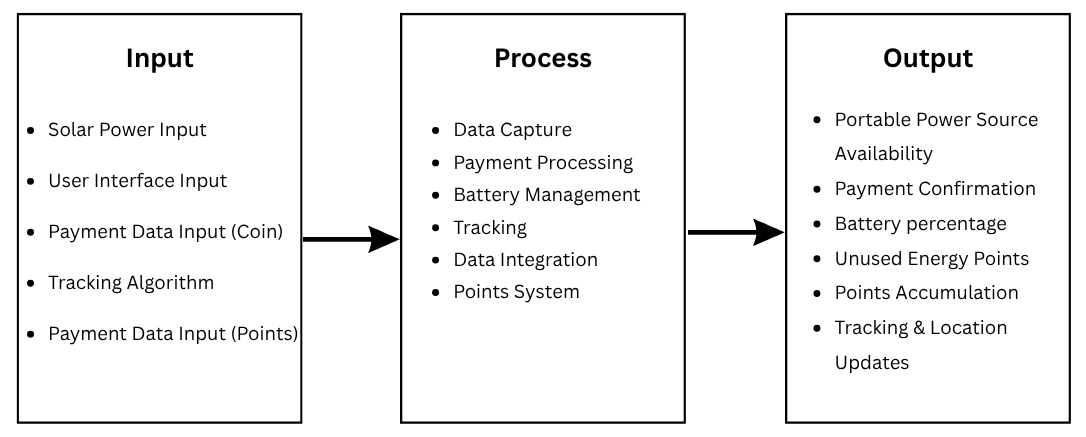
\includegraphics[width=1\textwidth]{figures/theoretical.png}
\end{figure}

Figiure 2.1 explains how the solar-powered rental station works from input to output. Inputs are what the system receives: solar energy that charges the main batteries, user actions on the screen or buttons, coins or points used for payment, and location data from GPS/GSM for tracking. The system then processes these inputs. It captures the user’s choice, checks and records the payment, manages the batteries by charging them and checking their levels, and updates each unit’s location. It also combines all this information so everything stays in sync, and it runs the points feature so unused energy can turn into rewards.

After processing, the system produces clear outputs that users and operators can see. It shows which portable power sources are available to rent, confirms that the payment went through, and displays the battery percentage of each unit before checkout. It also updates the user’s points, both the unused-energy points earned and the total points saved, and keeps the tracking information current, so rented units can be monitored in real time. This flow makes the station easy to use, transparent, and secure.


\section{Conceptual Framework}

\begin{figure}[H]
	\centering
	\caption{Process flow on how the system operates}
	\label{fig:conceptualfra}
	\includegraphics[width=1\textwidth]{figures/conceptual framework.png}
\end{figure}


Figure 2.2 illustrates the step-by-step process of how the proposed system functions, beginning with energy harvesting and ending with user access to the detachable power source. The process starts when photovoltaic (PV) panels capture solar energy and convert it into electricity. This electricity is then stored in the LiFePO4 battery, ensuring a reliable and long-lasting power supply. To make the stored energy usable for different devices, the system employs an inverter, which converts the direct current (DC) from the battery into alternating current (AC). Next, the ESP32 microcontroller, integrated with IoT mechanisms, monitors and manages the flow of energy. Through this control unit, real-time data such as battery charge level and system status can be tracked. Supporting modules such as GPS (for location tracking) and GSM (for wireless communication) enhance the monitoring and management of the system, particularly for rented power sources. For the rental mechanism, the system is equipped with a coin slot or app-based access system that unlocks the detachable power source through a solenoid lock. Once accessed, the user can rent and carry the power source for portable use, such as charging appliances or gadgets during power interruptions. The accompanying mobile application provides the renter with real-time updates on the battery level, usage duration, and system availability. Lastly, once the power source is returned, the system resets and recharges through solar harvesting, making it ready for the next user. This cyclical process ensures that the system remains sustainable, user-friendly, and reliable for communities experiencing frequent and unscheduled power interruptions.

\subsection{Schematic Diagram}

\begin{figure}[H]
	\centering
	\caption{Research Variables and Their Relationships}
	\label{fig:schematic}
	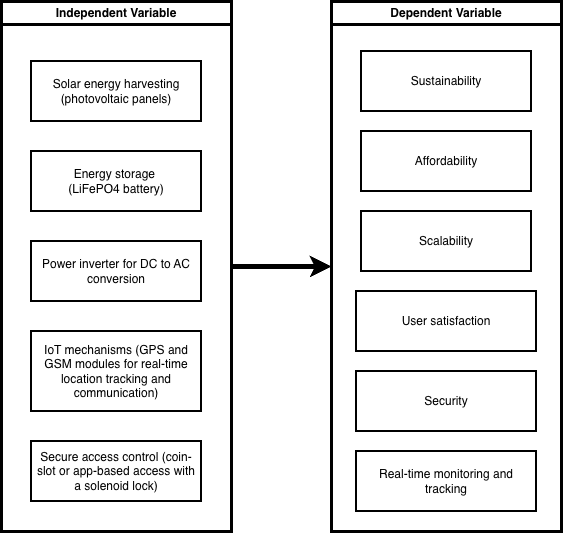
\includegraphics[width=0.8\textwidth]{figures/schematic.png}
\end{figure}

Figure 2.3 presents the independent and dependent variables, along with their relationship. The system integrates photovoltaic (PV) panels for solar energy harvesting, a process that involves capturing sunlight and converting it into usable electrical energy. The harvested solar energy is then stored in a \ce{LiFePO4} battery. Once stored, the direct current (DC) energy stored in the \ce{LiFePO4} battery is converted into alternating current (AC) by the power inverter. This conversion is essential since most household appliances and devices operate on AC power. Through this process, the system ensures a stable and usable power supply for various common electrical loads. The system also incorporates a GPS module, which continuously gathers satellite signals to provide real-time location data. This enables effective tracking and monitoring of the rented power sources. Simultaneously, the GSM module facilitates communication between the system and the administrator by transmitting data through cellular networks. It allows the system to send notifications, updates, and alerts to users in real time. To regulate user access, the system employs a secure payment mechanism. Before using the power source, users must make a payment through a coin-slot or app-based interface. Once payment is verified, the solenoid lock releases the detachable power source, ensuring that only authorized users can access it.

The dependent variables represent the measurable outcomes influenced by the performance of the solar-powered rental station. Sustainability pertains to the system’s capacity to maintain consistent and reliable operation over time through the use of renewable solar energy. It is evaluated based on the efficiency of energy generation, storage, and utilization under varying environmental conditions. Affordability refers to the system’s level of cost-effectiveness and economic accessibility, determining whether the rental fees, maintenance requirements, and operational expenses make it a viable and practical energy alternative during power outages. Scalability concerns the system’s potential to be expanded, replicated, or adapted for use in various communities or environments without compromising its cost efficiency or operational performance. User satisfaction measures how end-users perceive the system’s reliability, convenience, and overall usability. It is assessed through user feedback and usability evaluations focusing on accessibility, charging efficiency, and ease of operation. Security relates to the effectiveness of the system in safeguarding its physical components and digital data from unauthorized access, tampering, or misuse. Finally, real-time monitoring and tracking refer to the system’s capability to collect, transmit, and present accurate and timely data on power usage, battery status, and equipment location through the integration of IoT modules. Collectively, these dependent variables define the system’s efficiency, practicality, and long-term sustainability as an alternative energy source for communities experiencing frequent power interruptions.

The relationship between the independent and dependent variables focuses on how the proposed solar-powered rental station with detachable power sources influences the system’s overall effectiveness and performance. As the independent variable, the solar-powered rental station—integrating solar energy harvesting, energy storage, power conversion, Internet of Things (IoT) mechanisms, and secure access control—serves as the central technological concept of the study. The design and integration of these components are expected to affect several dependent variables, including sustainability, affordability, scalability, user satisfaction, security, and real-time monitoring. In this relationship, the independent variable represents the proposed system, while the dependent variables represent the measurable outcomes that determine its efficiency and practicality. Proper design and operation of the solar-powered rental station are assumed to enhance sustainability through stable energy generation and storage, promote affordability by minimizing operational costs, and enable scalability for broader deployment. Furthermore, the integration of IoT-based monitoring and secure access control is anticipated to improve user satisfaction, system security, and data accuracy. Overall, the conceptual framework illustrates that the system’s effectiveness depends on how well the independent variable’s components contribute to achieving reliable, sustainable, and user-oriented energy access during power interruptions.

\section{Review of Related Studies}

\subsection{Design of a Solar-Based Portable Power Supply with Modular Battery System for the Dumagat Tribe in Norzagaray, Bulacan}

Access to reliable and sustainable energy is a critical issue in many rural and indigenous communities. One such community is the Dumagat tribe in Norzagaray, Bulacan, where there is a notable lack of access to electricity despite the usage of electronic devices like phones. Addressing this issue requires innovative solutions that not only meet their energy demands but also ensure sustainability and accessibility. 

In this context, Gozano et al. (2023) conducted a study on a solar-powered portable power supply designed to provide the Dumagat Tribe with basic energy needs. This system incorporated a solar panel, a modular battery pack, and an inverter, aimed at powering low-energy devices and addressing the tribe’s electricity needs. Using an Arduino data logger, the study measured the charging and discharging rates of the system, showing promising results while also identifying areas for improvement, such as the need for higher-capacity batteries and more efficient solar panels.

\subsection{Construction of a Portable Solar Power Supply for Household Appliances}

Oluwasegun et al. (2018) developed a portable solar power supply system designed to power household appliances, offering a sustainable, eco-friendly alternative to traditional non-renewable energy sources. The system consists of a solar panel, a charge controller, a 12V lead-acid battery, a pure sine wave inverter, and an Arduino phase for voltage monitoring. The system was tested with household appliances such as a 300W electric blender and a 300W electric kettle, demonstrating its ability to provide reliable power. The solar panel efficiently converts sunlight into electricity, which is stored in the battery for use when solar energy is unavailable, providing a continuous energy supply.

The portable solar power system was able to power household appliances effectively, with minimal voltage drop during use, ensuring its practicality and dependability. By using solar energy, the system reduces electricity costs and promotes environmental sustainability by lowering greenhouse gas emissions. The use of a pure sine wave inverter ensures stable and high-quality power for sensitive appliances. Oluwasegun et al. (2018) concluded that this system offers a cost-effective, clean energy solution for households, though further enhancements are needed to support higher electrical loads for more extensive applications.

\subsection{Emergency Solar Portable Power Supply}

The "Emergency Portable Solar Power Supply" study by Ramly et al. (2019) explored the development of a portable solar power system designed to provide electricity in areas without reliable grid access, particularly during power outages. The system utilizes solar photovoltaic (PV) technology to convert sunlight into electricity, which is stored in a battery for later use. Key components of the system include solar panels, batteries, charge controllers, inverters, and a microcontroller with Bluetooth functionality for remote monitoring. The study emphasizes the importance of sizing the solar panels and batteries properly to ensure a consistent energy supply, particularly in off-grid or emergency situations. By harnessing renewable solar energy, the system reduces reliance on fossil fuels and contributes to environmental sustainability. The solar panels used in the system have an efficiency rating of around 15-18%.

\subsection{Portable Solar-Station with Integrated Battery Management and Load Monitoring System}

Abdur et al. (2024) describe the development of a portable solar-powered station designed for disaster response, offering a 200W output using a 2x2 array of 50W solar panels. The system integrates a battery management system (BMS) and load monitoring mechanism (LMM), providing power for essential needs such as lighting, mobile device charging, and medical equipment in emergency situations. Replacing diesel generators reduces environmental pollution and noise, offering a sustainable, clean energy solution in areas with limited infrastructure. Its compact design allows easy transportation to disaster zones, making it an effective tool for providing reliable power where it’s needed most.

The system also features an MPPT solar charge controller, optimizing energy efficiency and extending battery life by preventing overcharging and undercharging. The design incorporates Nanton YIDA YD-W50 Monocrystalline solar panels and a 12V 80Ah lead-acid battery, ensuring reliable energy storage. Abdur et al. (2024) conclude that this portable solar station provides a cost-effective, low-maintenance, and environmentally sustainable alternative to traditional diesel generators, making it a practical solution for disaster-prone regions.

\subsection{Solar Powered Mobile Power Bank Systems}

Solar-powered mobile charging systems offer a sustainable solution for powering devices during power interruptions and disasters. The research by Abdur et al. (2024) focuses on a Solar-Powered Portable Power Bank designed for mobile phones, using solar energy to charge a battery, which in turn provides power through a USB port. This system is particularly useful in disaster events and remote areas with limited electricity. The system utilizes two 6V solar panels to charge a 12V battery, with a microcontroller monitoring the battery’s charge level and controlling relay circuits to ensure safe charging.  LEDs display the battery charge level, offering a user-friendly interface for monitoring.

The proposed system has multiple advantages, including reducing reliance on traditional power sources and providing a reliable charging solution in emergencies. It addresses environmental concerns by utilizing renewable energy, minimizing pollution compared to conventional power generation methods. The microcontroller ensures efficient charge flow and protects the system from damage caused by overcharging or voltage fluctuations. Abdur et al. (2024) conclude that for optimal performance, the system requires direct sunlight and proper placement of the solar panels. The design can be improved by enhancing its portability and ensuring better protection for the mobile devices and battery, making it a practical and eco-friendly alternative to traditional charging methods.

\subsection{Multiport Universal Solar Power Bank}

Altelmessani et al. (2024) introduce the concept of a Multiport Universal Solar Power Bank, designed to harness solar energy for a portable power supply. This device aims to address critical needs in emergency situations and recreational activities like camping, especially in remote areas where access to electricity is limited. Equipped with solar panels for efficient energy absorption, the power bank offers both DC and AC outputs, making it versatile enough to charge a wide range of electronic devices. The project emphasizes the importance of sustainability, using renewable resources to reduce reliance on non-renewable energy sources and provide a reliable, eco-friendly power source.

The system is capable of powering various appliances, including small household electronics, portable fans, lights, and mobile devices, with an AC output of up to 400W and a battery capacity of 20,000mAh. It also incorporates safety features to protect against overcharging, overheating, and other risks, ensuring both user safety and device longevity. The study highlights the project’s compact and lightweight design, making it ideal for on-the-go use, such as in emergencies or outdoor activities. By focusing on energy independence and environmental sustainability, the project contributes to reducing environmental impact while offering a reliable and versatile energy solution.

\subsection{Portable Power Supply Design with 100 Watt Capacity}

Zakri et al. (2021) developed a portable solar power supply design with a 100W capacity, aimed at providing sustainable energy in areas with limited electricity access. The system utilizes solar cells and a transformer to store energy in batteries with capacities of 20Ah, 60Ah, and 100Ah. The solar-powered generator can charge devices like lamps, laptops, LED televisions, and fans, supporting electrical loads under 100 watts for up to 12 hours. The system includes a Solar Charge Controller (SCC) to prevent overcharging, ensuring battery safety and longevity. The design is portable, easy to operate, and suitable for off-grid locations such as plantations or rural areas.

The tool's efficiency depends on the battery capacity and weather conditions. For example, charging the 20Ah battery takes about 5 hours under optimal sunlight, while larger batteries (60Ah and 100Ah) require more than one day to fully charge. This design is versatile, offering both AC and DC outputs, and is equipped with an LCD for voltage display, as well as safety features such as overcharge protection. Zakri et al. (2021) conclude that this portable power supply offers a practical, environmentally friendly solution for off-grid applications, with the flexibility to charge batteries via solar energy or electrical sources.

\subsection{Design and Development of Portable StandAlone Solar Power Generator }

Prathiba et al. (2020) developed a portable, standalone solar power generator designed to replace diesel generators with a sustainable, eco-friendly solution. The system integrates a solar panel, a battery, a bidirectional buck-boost converter, and an inverter, all supported by a Maximum Power Point Tracking (MPPT) algorithm for optimal efficiency. The generator provides a green energy source to meet load requirements and stores excess energy in a battery for use when solar energy is unavailable. The bidirectional converter enhances battery charging efficiency and ensures regulated DC voltage output, while the MPPT algorithm maximizes power extraction from the solar panel to improve overall system performance.

The portable solar generator utilizes a bi-directional converter and MPPT to achieve high efficiency, allowing it to charge and discharge a 12V lead-acid battery. The system is capable of powering both DC and AC loads, using a push-pull full-bridge inverter to drive AC devices. The system is designed for off-grid applications, including emergency situations and areas without access to electricity. The study emphasizes the system's compact design, cost-effectiveness, and potential for use in relief camps and remote locations. The project demonstrates a practical and portable renewable energy solution for sustainable power generation in diverse applications, especially in areas with limited access to the grid.

\subsection{A solar-powered multi-functional portable charging device (SPMFPCD) with internet-of-things (IoT)-based real-time monitoring- An innovative scheme towards energy access and management}

Rehman et al. (2024) propose a solar-powered multi-functional portable charging device (SPMFPCD) with IoT-based real-time monitoring, designed to address the growing need for reliable and versatile energy solutions across various sectors, including transportation, communication, and emergency services. The device integrates a highly efficient solar panel, a charge controller, sensors, and an IoT module for real-time monitoring of power parameters. This innovative system supports diverse applications, such as emergency medical device charging, outdoor adventures, disaster management, and public spaces. The IoT capabilities provide continuous monitoring, ensuring efficient operation and proactive maintenance, enhancing the reliability and scalability of the system.

The study emphasizes the significance of integrating advanced technologies, such as IoT-driven battery energy storage system (BESS) health monitoring, to optimize the performance and lifespan of the system. The study also conducted an economic and environmental impact assessment, showing the feasibility and sustainability of widespread SPMFPCD deployment. The proposed system demonstrated competitive cost-effectiveness, with a low cost of electricity and minimal annual operating costs. The integration of renewable energy sources like solar power and the IoT-based health monitoring system positions the SPMFPCD as a promising solution for providing accessible, environmentally friendly energy in various settings, highlighting its potential to contribute to sustainable energy management and community empowerment.

\subsection{Development of a Low Cost Portable Hydro and Wind Power as Emergency Power Source}

The study of low-cost portable hydro and wind power system as an emergency power source by Supardi et al. (2020) explored the development of a low-cost portable hydro and wind power system as an emergency power source. The system is designed to provide power for recharging essential equipment such as mobile phones, radios, and emergency lights, which are essential during prolonged outdoor activities or power outages. This system can be implemented in remote areas with fluctuating water flows, making it an ideal solution for communities with limited access to electricity. The study found that the portable hydropower system, when coupled with wind power, could generate reliable electricity. These findings support the integration of renewable energy sources in off-grid locations, where accessibility to traditional power infrastructure is limited, and emphasize the importance of efficient turbine and generator design for portable power generation.

\subsection{Development of Portable Solar Storage Device}

Roslan et al. (2019) developed a portable solar storage (PSS) device designed to address the increasing demand for sustainable and portable power sources. The PSS is tailored for outdoor activities, such as hiking, camping, and climbing, providing a portable solution for charging electronic devices. The system uses a 12V or 18V solar panel to charge a battery with 98W of energy storage. During testing, the system showed charging rates of 16.086 W/h for the 12V solar panel and 13.35 W/h for the 18V panel, demonstrating the effectiveness of solar energy harvesting. The PSS was capable of recharging devices with capacities up to 10,000mAh, offering a reliable power supply for small electronic gadgets.

The study highlights the advantages of using solar panels for off-grid applications, noting that the PSS is ideal for areas with ample sunlight, such as Malaysia. The device’s efficiency was calculated at 12.75\%, with the system capable of charging devices like phones, smartphones, and power banks. However, the study also found limitations in charging larger devices with the 12V solar panel. Roslan et al. (2019) concluded that while the PSS provides an environmentally friendly and practical solution for outdoor power needs, further improvements in solar panel capacity and battery efficiency are needed to enhance its performance for higher power demands.

\subsection{Renewable Energy from Solar Panels: A Study of  Photovoltaic Physics and Environmental Benefits}

Jaiswal (2023) provides an in-depth analysis of solar energy’s growing role in the global energy transition, focusing on its environmental, economic, and technological advantages. The study highlights that global solar photovoltaic (PV) capacity reached about 1,059 gigawatts by 2021, reflecting rapid adoption and its significant contribution to reducing greenhouse gas emissions. Technological advancements, such as bifacial and perovskite solar cells, have increased the efficiency and affordability of solar power, making it more accessible. The research also stresses the importance of supportive policies and regulatory frameworks in promoting solar energy deployment.

The environmental benefits of solar power are significant, with Jaiswal (2023) noting that solar energy could reduce up to 80\% of greenhouse gas emissions by 2050. Additionally, the integration of solar energy with energy storage systems is essential for improving reliability and addressing challenges related to intermittency. The study concludes that solar energy plays a crucial role in achieving sustainable development, reducing climate change impacts, and driving economic growth. With ongoing technological advancements and effective policies, solar power is set to be a key component of the future energy system.

\subsection{Power Consumption of Household Appliances }

Power consumption patterns in households are significantly influenced by the frequency and duration of appliance usage. Pulvera (2021) found that household appliances such as televisions, electric fans, and refrigerators are among the most frequently used devices, contributing considerably to total electricity consumption. The results revealed that the television set operates for an average of forty-four (44) hours per week, followed by the electric fan with fifty-one (51) hours, and the refrigerator with one hundred five (105) hours of usage weekly. These appliances are commonly prioritized for their essential roles in providing comfort, entertainment, and food preservation within the household.

Pulvera (2021) further emphasized that electricity usage is affected by several factors, including low voltage supply, appliance wattage, power interruptions, standby power, and user behavior. Among these, user awareness and proper energy management play a crucial role in reducing unnecessary power consumption. The continuous use of high-demand appliances such as electric fans and refrigerators, especially in tropical climates like the Philippines, highlights the dependence of households on these devices for maintaining comfort during hot weather and ensuring food preservation. Consequently, understanding the frequency of appliance use helps identify energy-saving opportunities and promote consumer awareness.

\subsection{Electricity Distribution and Supply Authority}

Battery selection plays a critical role in optimizing the performance and sustainability of photovoltaic (PV) systems. According to the Electricity Distribution and Supply Authority (EDSA, 2024) under the Government of Sierra Leone, three major battery options are typically considered in solar power applications—Flooded Lead Acid, Sealed Lead Acid (SLA), and Lithium Iron Phosphate (\ce{LiFePO4}). The study highlighted that \ce{LiFePO4} batteries are preferred for the Regional Emergency Solar Power Intervention (RESPITE) Project due to their superior efficiency, longevity, and environmental advantages.

\ce{LiFePO4} batteries are generally more energy-efficient, allowing for greater energy utilization and reduced losses during charging and discharging. In contrast, SLA batteries exhibit lower efficiency, which can result in higher energy wastage. Additionally, \ce{LiFePO4} batteries support a higher depth of discharge (DoD), enabling deeper energy use without significantly affecting their lifespan. This characteristic makes them more suitable for daily solar energy cycling compared to SLA batteries, which tend to degrade faster under similar conditions.

Another major advantage of \ce{LiFePO4} technology is its longer cycle life. The EDSA (2024) report notes that \ce{LiFePO4} batteries can endure more charge-discharge cycles before their performance diminishes, offering better long-term reliability. They also possess higher energy density, meaning they can store more energy in a smaller physical footprint—an important factor when space constraints exist in solar installations.

In terms of maintenance, \ce{LiFePO4} batteries are maintenance-free, unlike SLA batteries which often require periodic electrolyte checks and refilling. While \ce{LiFePO4} batteries have a higher upfront cost, they compensate with lower operational and maintenance expenses throughout their lifespan. From an environmental perspective, \ce{LiFePO4} batteries are also less harmful and easier to dispose of or recycle compared to lead-acid types, which generate toxic emissions during recycling.

\subsection{Assessing the Impact of Power Outages on Appliances of Farmers and Fisherfolks in Selected Barangays of Cawayan, Masbate, Philippines: Basis for a Proposed Extension Program}

Frequent power interruptions have long been a challenge in rural communities, particularly among farmers and fisherfolk who depend on electricity for household and livelihood activities. The study aimed to determine the impact of frequent power interruptions on the appliances and economic well-being of residents in selected barangays of Cawayan, Masbate. Employing a descriptive research design, the researchers gathered data from 266 respondents through paper surveys and face-to-face interviews to assess the frequency, duration, and effects of power interruptions. Findings revealed that almost all respondents experienced power interruptions lasting three to four hours, leading to increased electricity consumption and higher bills. Refrigerators and televisions were the most power-consuming appliances, and there was significant damage to appliances, especially bulbs, as well as disruptions to income-generating activities. The study results showed that many respondents had an annual income of less than \textpeso18,200, which was considered low and may have resulted in difficulty in paying high bills brought by power outages. All respondents relied on the power grid as their source of electricity, and power interruptions were a common occurrence. The data revealed that 97.7\% of respondents experienced power interruptions, with 51.1\% experiencing 3-4 hours of interruption. Almost all respondents claimed that power interruption increased their electric consumption and bill, and 56\% were not satisfied with their electric bill when there was a power interruption. It was concluded that unreliable electricity supply and lack of maintenance significantly affect low-income households that rely solely on the power grid as their source of electricity. The study recommended strengthening local power infrastructure and promoting renewable energy education through a proposed extension project that trains communities in the use of solar energy as a sustainable and reliable alternative to the current power grid system. This helps reduce air pollution and climate change while building the capacity of farmers and fishers to adapt to these changes.

\subsection{Solar-Powered Coin-Operated Mobile Charging Station for Sustainable Energy Access and Resilience}

The increasing demand for sustainable and accessible energy has driven innovations that utilize renewable sources to meet electricity needs in both urban and rural areas. The study by Catalan, Occeña, Gabion, Occeña, and Ejar (2023) aimed to develop a solar-powered, coin-operated mobile charging station designed to provide continuous off-grid power using photovoltaic (PV) technology. Employing a developmental research approach, the researchers designed, fabricated, and tested a prototype equipped with solar panels and an integrated storage battery system capable of charging multiple mobile devices for both commercial and emergency purposes. The results demonstrated that the charging station effectively powered various mobile gadget models with no compatibility issues, maintained stable operation even under limited sunlight, and offered cost efficiency through its low maintenance and sustainable design. Furthermore, the system contributed to reducing carbon emissions and supported the green technology initiatives of Guimaras State University. It was concluded that the solar-powered charging station is a practical and eco-friendly innovation that promotes energy resilience in communities affected by power outages. The study recommended installing such systems in strategic locations for communal purposes and remote areas, integrating security features to prevent misuse, and conducting further research to enhance its technological design and promote the widespread adoption of renewable energy solutions.

\subsection{Synthesis}

The reviewed literature highlights the progress made in solar-powered portable energy systems, especially for off-grid communities facing frequent power interruptions and power emergencies. Studies like those by Gozano et al. (2023), Oluwasegun et al. (2018), and Ramly et al. (2019) developed solar-based systems that integrated photovoltaic panels, charge controllers, batteries, and inverters. However, these systems often lacked sufficient energy storage capacity, limiting their ability to provide continuous power for communities that rely heavily on energy for daily appliances such as refrigerators and fans. Studies by Abdur et al. (2024) and Altelmessani et al. (2024) incorporated more advanced energy management through battery monitoring and load management systems but still did not fully address the integration of high-capacity energy storage and secure access for users. The gap in addressing these challenges highlights the need for a more efficient and accessible solar energy system for communities affected by power disruptions.

A significant gap in the existing literature lies in the choice of energy storage solutions. Many studies employed Lead-Acid batteries, which are still common in many solar power systems. For example, Oluwasegun et al. (2018) used a 12V Lead-Acid battery, which is cheaper but comes with limitations, including lower efficiency, shorter cycle life, and higher maintenance requirements. Lead-Acid batteries are typically less efficient, with a cycle life of about 500 to 1,000 cycles. In contrast, the proposed system utilizes LiFePO4 (Lithium Iron Phosphate) batteries which is a better  alternative. According to EDSA (2024) and Zakri et al. (2021), LiFePO4 batteries offer several advantages, including a much higher cycle life (more than 2,000 cycles), greater depth of discharge (DoD), and better overall efficiency, making them ideal for systems that undergo frequent charge-discharge cycles. These batteries are also more environmentally friendly and require less maintenance than their lead-acid counterparts. The LiFePO4 battery selected for the proposed system offers reliable energy storage with a high energy density, ensuring longer-lasting and more sustainable power for the solar-powered rental station.

Additionally, a notable gap in the literature is the lack of secure, rental-based access mechanisms for solar energy systems. While studies like Catalan et al. (2023) explored solar-powered coin-operated charging stations, they primarily focused on mobile charging rather than integrated power solutions for household or community use. The current study addresses this gap by incorporating a coin-slot mechanism with a solenoid lock for secure, pay-per-use access, ensuring that only authorized users can access the stored energy. Moreover, the integration of IoT-based monitoring through the ESP32 microcontroller, GPS, and GSM modules provides real-time tracking of battery levels, usage statistics, and system status, which has not been fully explored in previous research. Rehman et al. (2024) highlighted the use of IoT for real-time monitoring in solar-powered devices, but their research focused on charging stations for mobile devices rather than community-based energy solutions. The integration of a mobile app for monitoring battery charge levels and energy consumption ensures that users have full visibility into the system’s performance.

Furthermore, the proposed system's combination of a 2x2 solar panel array, LiFePO4 battery, MPPT charge controller, and AC inverter ensures that the system is capable of powering small to medium-sized appliances, such as refrigerators and fans, which are commonly used in Filipino households as noted in the studies by Pulvera (2021) and Masbate (2024). This integrated approach addresses a crucial need for accessible and reliable energy solutions in communities that frequently face power interruptions. The system’s scalability and eco-friendly design, driven by high-capacity LiFePO4 batteries, secure rental features, and smart monitoring systems, provide a comprehensive solution that builds on existing research while filling the gap in accessible and sustainable solar energy solutions for off-grid communities.


}